\chapter{Study}

\section{Motivations}  

%From our exploratory study, we were able to obtain a significant but weak effect between disclosing the source and the levels of trust marked by readers towards an article.

% We also observed trends that suggested an interaction between disclosing the source and the reading level of a story.

% However, the study faced several limitations: first, we did not obtain enough samples to show a statistically significant result for interactions between source and reading level.

% Furthermore, multiple levels of independent variables (ie: 5 levels for input source) made modeling complex and the results less clear.

% The dataset was also unbalanced and sparse (ie, because of large numbers of input variables we did not have complete representation for each category, such as high, low, and mid-reading level stories for every outlet and topic). We tried to control for those factors by randomization, however it made more difficult to analyze specific correlations between source and trust.

% To further explore the interaction between disclosing the source and the reading level of the story, we set up another crowdsourcing experiment on CrowdFlower, this time targeting this specific interaction, to see if there is a significant effect between the two, detailed in the following chapter.
 

This study focused on two main hypotheses:

\begin{itemize}
  \item H1
  \item H2
\end{itemize}


\section{Experimental Design}

For the second study, our experiment was revised to have a 4 x 2 mixed-factorial design.
In this study, reading level of articles and candidates featured in the articles were treated as within-subject variables, and the source of the story between-subjects.

\begin{center}
\begin{table}
\begin{tabular}{ | m{10em} | m{7em}| m{7em} | m{7em} | m{7em} | } 
 \hline
  & \textbf{Source: None} & \textbf{Source: AP} & \textbf{Source: Fox} & \textbf{Source: CNN} \\
 \hline
 \textbf{High Reading Level} & Clinton, Cruz, Sanders, Trump & Clinton, Cruz, Sanders, Trump & Clinton, Cruz, Sanders, Trump & Clinton, Cruz, Sanders, Trump  \\ 
 \textbf{Low Reading Level} & Clinton, Cruz, Sanders, Trump & Clinton, Cruz, Sanders, Trump & Clinton, Cruz, Sanders, Trump & Clinton, Cruz, Sanders, Trump \\ 
 \hline
\end{tabular}
\caption{Main Study Design}
\label{study2}
\end{table}
\end{center}
%\newpage

% \begin{itemize}
%   \item Source (4 levels: None, AP, CNN, Fox)
%   \item Candidate (4 levels: Clinton, Cruz, Sanders, Trump)
%   \item Reading Level (2 levels: High, Low)
% \end{itemize}

This time, we reduced the number of stories to N=8, and also changed reading level from a 3-level to 2-level variable (low, high) for clarity.

Most significantly, since we observed some significant effect from disclosing source to the reader in Study 1, we added a manipulation in this experiment to further study the effect of revealing the source:

Following Baum's research in showing the effects of media brands and reader bias by manipulating reported brands, all eight stories in Study 2 were in fact written by the Associated Press, however, we manipulated the source shown to the reader \cite{baum2008eye}. In group A, readers were shown the headline and text of the story with no other context. In group B, readers were additionally shown that the story was from the Associated Press (true label). In groups C and D, readers were shown that the story was from CNN and Fox News, respectively.

This setup was created to eliminate some of the confounding effects from using stories from different sources (writing style, focus of content, slant, etc.), while directly observing the effect of revealing a specific source to the reader. The Associated Press was chosen as the source of the stories as it is the highest circulation newswire service in the United States, and has 14,000 members that use its content \cite{apFAQ}. Notably, both CNN and Fox News publish content in full or part from the Associated Press, although the specific stories chosen had not been published in full by either to avoid bias.

We removed the favorability question from Study 1 (as the 3-point scale did not yield significant results), instead asking the reader more directly about media bias by ranking the fairness of the story on a 5-point Likert scale. The trustworthiness question from Study 1 was kept, also on the same 5-point Likert scale.


\subsection{Dataset} 
Eight stories were chosen for this study: two (high and low reading level) per candidate. All eight stories were written by reporters from the Associated Press (although they may have been republished elsewhere).

Reading level cutoffs were made by taking the bottom and top 25\% percentile of Flesch-Kincaid scores for each candidate. From stories written by the Associated Press that made the cutoff, we formed pairs of high and low reading level stories from each topic. The topic with the highest distance between reading level in the pair was chosen for each candidate.

% put histograms of reading level with cutoff lines

 
 
 
\subsection{Survey}


\begin{figure}[h!] 
\centering
  \frame{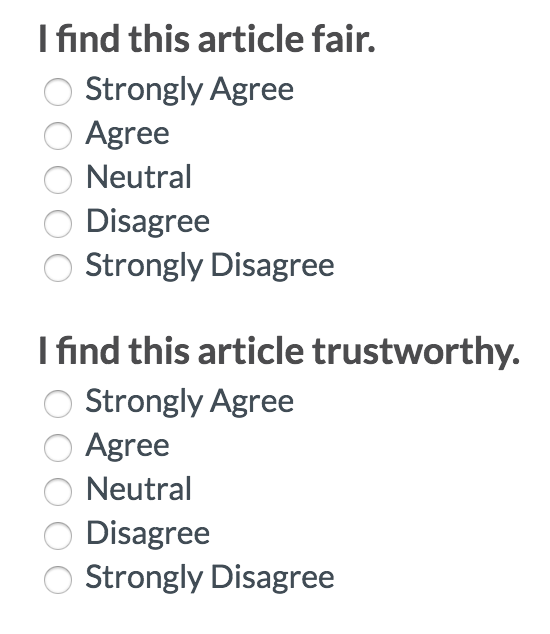
\includegraphics[width=0.45\textwidth]{study2_qs}}
  \caption{Survey Questions for Study 2}
\end{figure}



Demographics
What is your gender?
 Male
 Female
 Other
What is your age?
 18-29
 30-49
 50-64
 64+
What is your political party affiliation?
 Democrat
 Republican
 Independent/Other
 No Affiliation
If the election were tomorrow, I would vote for…
 Hillary Clinton
 Bernie Sanders
 Donald Trump
 Ted Cruz
 John Kasich
 Other
 Might not vote
Have you read any of the stories above before this study?
 Yes
 No
 Might have, but I am not sure


 % when we removed people who might have already read stories, no sig diff results in analysis.



% just pics etc.
\subsection{Quality Control}

As in the first study, users were filtered by minimum time taken to complete the task. Again, only Level 3 workers were chosen from Crowdflower, and users from Study 1 were forbidden to complete tasks in Study 2. 

Because Study 2 presented a longer task of reading 8 versus 5 news stories, we set a longer minimum time of 6 minutes to complete the task. A payment of \$0.80 per survey was given based off guidelines by MIT \cite{COUHES-turk}.

The average response time for the task was 09:20 min.

\section{Analysis}


\subsection{Demographics}
basic demographics of voters.

\subsection{Trends}
descriptive analytics of fairness and trust.



%Why did you choose trust and fairness?

 
% How did you control for quality?

  
% What kind of people signed up for your study?

% How did you recruit them? What was their incentive?

% What kind of effects were you looking for?
 
% What kind of effects did you find?

\section{Conclusions}

How do your trustworthiness findings line up with the findings from Pew surveys and prior work? What hypotheses did you verify from prior work?

\section{Limitations}

Just 8 stories I know
Yes the diff candidates had diff topics i know
we could have included all candidates
